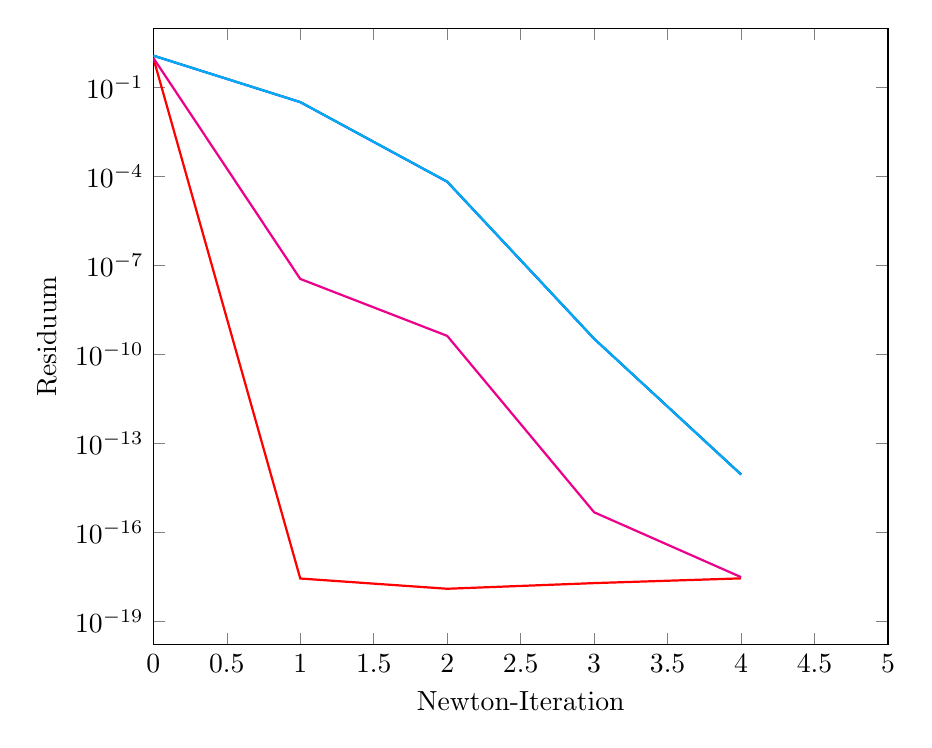
\begin{tikzpicture}[every plot/.append style={thick}] 
\begin{axis}[ 
label style={font=\normalsize}, 
xlabel={Newton-Iteration}, 
ylabel={Residuum}, 
xmin=0, xmax=5, 
ymode=log, 
ymin=0, ymax=10, 
width=0.9\textwidth, 
grid style=dashed, 
] 
\addplot[ 
color=blue, 
] 
coordinates { 
(0, 1.19e+00)(1, 3.22e-02)(2, 6.63e-05)(3, 3.34e-10)(4, 8.81e-15)}; 
\addplot[ 
color=red, 
] 
coordinates { 
(0, 1.00e+00)(1, 2.73e-18)(2, 1.23e-18)(3, 1.91e-18)(4, 2.76e-18)}; 
\addplot[ 
color=cyan, 
] 
coordinates { 
(0, 1.19e+00)(1, 3.22e-02)(2, 6.68e-05)(3, 3.35e-10)(4, 8.69e-15)}; 
\addplot[ 
color=magenta, 
] 
coordinates { 
(0, 1.00e+00)(1, 3.49e-08)(2, 4.18e-10)(3, 4.68e-16)(4, 3.03e-18)}; 
\end{axis} 
\end{tikzpicture} 
